\documentclass{standalone}
\usepackage{tikz}
\usetikzlibrary{patterns, positioning}
\usepackage[sfdefault]{ClearSans} %% option 'sfdefault' activates Clear Sans as the default text font
\usepackage[T1]{fontenc}

\begin{document}
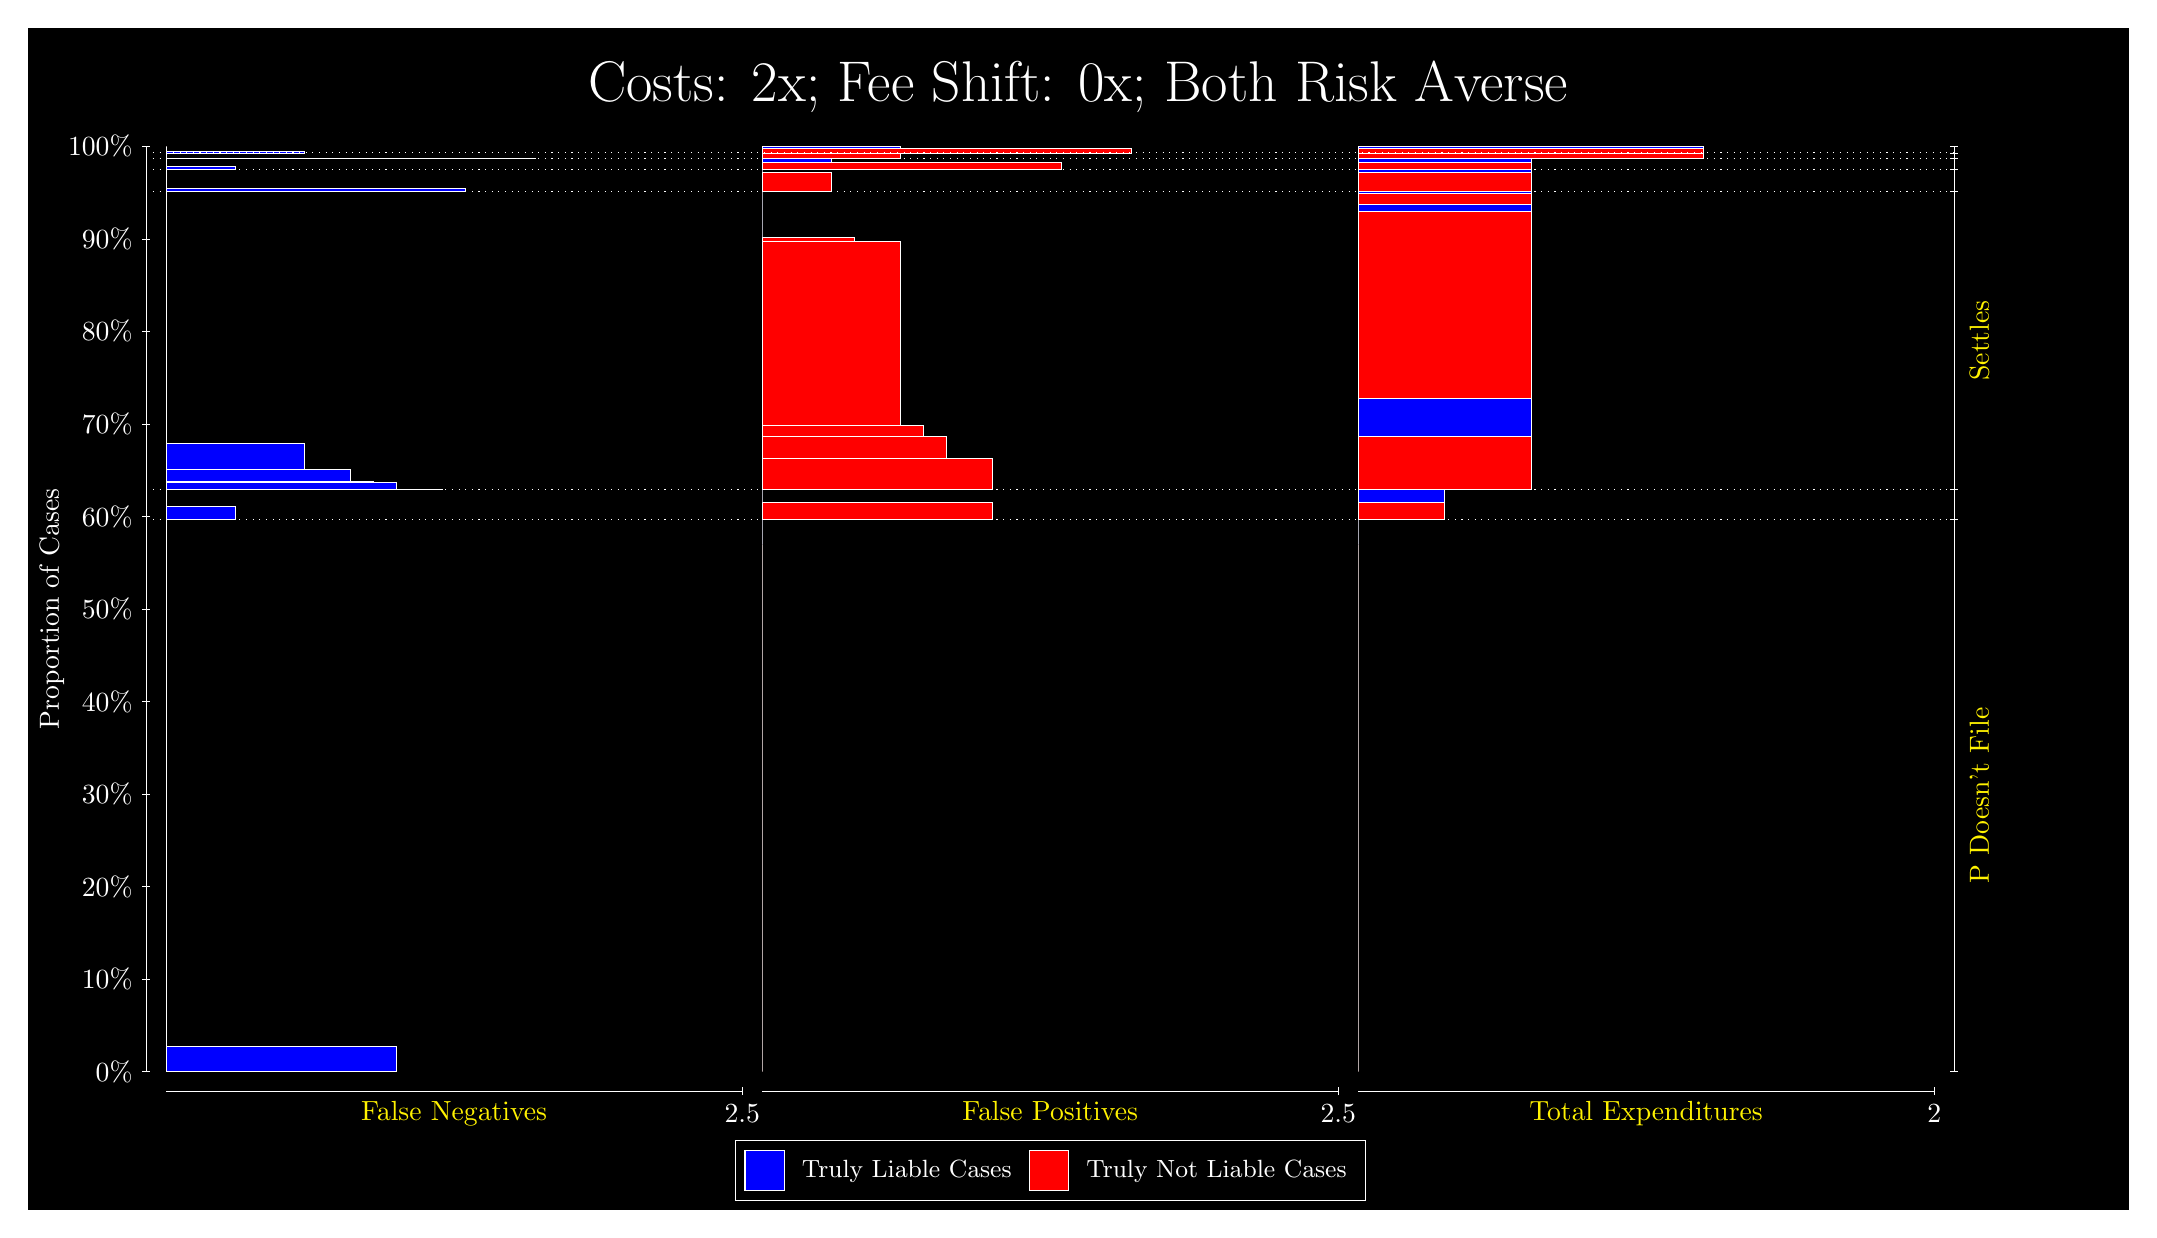
\begin{tikzpicture}
\draw[fill=black] (0,0) rectangle (26.667,15);
\draw[text=white] (0,13.5) rectangle (26.667,15) node[midway] {\huge Costs: 2x; Fee Shift: 0x; Both Risk Averse};
\draw[white, very thin] (1.5,1.75) -- (1.5,13.5);
\node[rotate=90, text=white, anchor=center] at (0.3, 7.625) {Proportion of Cases};
\draw[white, very thin] (1.45,1.75) -- (1.55,1.75);
\node[text=white, anchor=east] at (1.45, 1.75) {0\%};
\draw[white, very thin] (1.45,2.925) -- (1.55,2.925);
\node[text=white, anchor=east] at (1.45, 2.925) {10\%};
\draw[white, very thin] (1.45,4.1) -- (1.55,4.1);
\node[text=white, anchor=east] at (1.45, 4.1) {20\%};
\draw[white, very thin] (1.45,5.275) -- (1.55,5.275);
\node[text=white, anchor=east] at (1.45, 5.275) {30\%};
\draw[white, very thin] (1.45,6.45) -- (1.55,6.45);
\node[text=white, anchor=east] at (1.45, 6.45) {40\%};
\draw[white, very thin] (1.45,7.625) -- (1.55,7.625);
\node[text=white, anchor=east] at (1.45, 7.625) {50\%};
\draw[white, very thin] (1.45,8.8) -- (1.55,8.8);
\node[text=white, anchor=east] at (1.45, 8.8) {60\%};
\draw[white, very thin] (1.45,9.975) -- (1.55,9.975);
\node[text=white, anchor=east] at (1.45, 9.975) {70\%};
\draw[white, very thin] (1.45,11.15) -- (1.55,11.15);
\node[text=white, anchor=east] at (1.45, 11.15) {80\%};
\draw[white, very thin] (1.45,12.325) -- (1.55,12.325);
\node[text=white, anchor=east] at (1.45, 12.325) {90\%};
\draw[white, very thin] (1.45,13.5) -- (1.55,13.5);
\node[text=white, anchor=east] at (1.45, 13.5) {100\%};

\draw[white, very thin] (24.457,1.75) -- (24.457,13.5);
\draw[white, very thin] (24.407,1.75) -- (24.507,1.75);
\node[anchor=west] at (24.407, 1.75) {};
\draw[white, very thin] (24.407,8.7605) -- (24.507,8.7605);
\node[anchor=west] at (24.407, 8.7605) {};
\draw[white, very thin] (24.407,9.1402) -- (24.507,9.1402);
\node[anchor=west] at (24.407, 9.1402) {};
\draw[white, very thin] (24.407,12.929) -- (24.507,12.929);
\node[anchor=west] at (24.407, 12.929) {};
\draw[white, very thin] (24.407,13.203) -- (24.507,13.203);
\node[anchor=west] at (24.407, 13.203) {};
\draw[white, very thin] (24.407,13.343) -- (24.507,13.343);
\node[anchor=west] at (24.407, 13.343) {};
\draw[white, very thin] (24.407,13.417) -- (24.507,13.417);
\node[anchor=west] at (24.407, 13.417) {};
\draw[white, very thin] (24.407,13.5) -- (24.507,13.5);
\node[anchor=west] at (24.407, 13.5) {};

\draw[white, very thin, fill=blue] (1.75,1.75) rectangle (4.6775,2.0648);
\draw[white, very thin, fill=red] (1.75,2.0648) rectangle (1.75,8.7605);
\draw[white, very thin, fill=blue] (1.75,8.7605) rectangle (2.6283,8.9258);
\draw[white, very thin, fill=red] (1.75,8.9258) rectangle (1.75,9.1402);
\draw[white, very thin, fill=blue] (1.75,9.1402) rectangle (5.2631,9.1456);
\draw[white, very thin, fill=blue] (1.75,9.1456) rectangle (4.6775,9.2276);
\draw[white, very thin, fill=blue] (1.75,9.2276) rectangle (4.3848,9.2523);
\draw[white, very thin, fill=blue] (1.75,9.2523) rectangle (4.092,9.3956);
\draw[white, very thin, fill=blue] (1.75,9.3956) rectangle (3.5065,9.7302);
\draw[white, very thin, fill=red] (1.75,9.7302) rectangle (1.75,12.929);
\draw[white, very thin, fill=blue] (1.75,12.929) rectangle (5.5558,12.961);
\draw[white, very thin, fill=red] (1.75,12.961) rectangle (1.75,13.203);
\draw[white, very thin, fill=blue] (1.75,13.203) rectangle (2.6283,13.246);
\draw[white, very thin, fill=red] (1.75,13.246) rectangle (1.75,13.343);
\draw[white, very thin, fill=blue] (1.75,13.343) rectangle (6.4341,13.349);
\draw[white, very thin, fill=red] (1.75,13.349) rectangle (1.75,13.417);
\draw[white, very thin, fill=blue] (1.75,13.417) rectangle (3.5065,13.44);
\draw[white, very thin, fill=red] (1.75,13.44) rectangle (1.75,13.5);
\draw[white, very thin, fill=red] (9.3189,1.75) rectangle (9.3189,8.4457);
\draw[white, very thin, fill=blue] (9.3189,8.4457) rectangle (9.3189,8.7605);
\draw[white, very thin, fill=red] (9.3189,8.7605) rectangle (12.246,8.9749);
\draw[white, very thin, fill=blue] (9.3189,8.9749) rectangle (9.3189,9.1402);
\draw[white, very thin, fill=red] (9.3189,9.1402) rectangle (12.246,9.5328);
\draw[white, very thin, fill=red] (9.3189,9.5328) rectangle (11.661,9.8183);
\draw[white, very thin, fill=red] (9.3189,9.8183) rectangle (11.368,9.9574);
\draw[white, very thin, fill=red] (9.3189,9.9574) rectangle (11.075,12.291);
\draw[white, very thin, fill=red] (9.3189,12.291) rectangle (10.49,12.339);
\draw[white, very thin, fill=blue] (9.3189,12.339) rectangle (9.3189,12.929);
\draw[white, very thin, fill=red] (9.3189,12.929) rectangle (10.197,13.171);
\draw[white, very thin, fill=blue] (9.3189,13.171) rectangle (9.3189,13.203);
\draw[white, very thin, fill=red] (9.3189,13.203) rectangle (13.125,13.3);
\draw[white, very thin, fill=blue] (9.3189,13.3) rectangle (10.197,13.343);
\draw[white, very thin, fill=red] (9.3189,13.343) rectangle (11.075,13.411);
\draw[white, very thin, fill=blue] (9.3189,13.411) rectangle (9.3189,13.417);
\draw[white, very thin, fill=red] (9.3189,13.417) rectangle (14.003,13.477);
\draw[white, very thin, fill=blue] (9.3189,13.477) rectangle (11.075,13.5);
\draw[white, very thin, fill=red] (16.888,1.75) rectangle (16.888,8.4457);
\draw[white, very thin, fill=blue] (16.888,8.4457) rectangle (16.888,8.7605);
\draw[white, very thin, fill=red] (16.888,8.7605) rectangle (17.986,8.9749);
\draw[white, very thin, fill=blue] (16.888,8.9749) rectangle (17.986,9.1402);
\draw[white, very thin, fill=red] (16.888,9.1402) rectangle (19.083,9.8183);
\draw[white, very thin, fill=blue] (16.888,9.8183) rectangle (19.083,10.296);
\draw[white, very thin, fill=red] (16.888,10.296) rectangle (19.083,12.677);
\draw[white, very thin, fill=blue] (16.888,12.677) rectangle (19.083,12.765);
\draw[white, very thin, fill=red] (16.888,12.765) rectangle (19.083,12.904);
\draw[white, very thin, fill=blue] (16.888,12.904) rectangle (19.083,12.929);
\draw[white, very thin, fill=red] (16.888,12.929) rectangle (19.083,13.171);
\draw[white, very thin, fill=blue] (16.888,13.171) rectangle (19.083,13.203);
\draw[white, very thin, fill=red] (16.888,13.203) rectangle (19.083,13.3);
\draw[white, very thin, fill=blue] (16.888,13.3) rectangle (19.083,13.343);
\draw[white, very thin, fill=red] (16.888,13.343) rectangle (21.279,13.411);
\draw[white, very thin, fill=blue] (16.888,13.411) rectangle (21.279,13.417);
\draw[white, very thin, fill=red] (16.888,13.417) rectangle (21.279,13.477);
\draw[white, very thin, fill=blue] (16.888,13.477) rectangle (21.279,13.5);
\draw[white, dotted] (1.5,8.7605) -- (24.457,8.7605);
\draw[white, dotted] (1.5,9.1402) -- (24.457,9.1402);
\draw[white, dotted] (1.5,12.929) -- (24.457,12.929);
\draw[white, dotted] (1.5,13.203) -- (24.457,13.203);
\draw[white, dotted] (1.5,13.343) -- (24.457,13.343);
\draw[white, dotted] (1.5,13.417) -- (24.457,13.417);
\draw[white, very thin] (1.75,1.5) -- (9.0689,1.5);
\node[text=yellow, anchor=north] at (5.4094, 1.5) {False Negatives};
\draw[white, very thin] (9.0689,1.45) -- (9.0689,1.55);
\node[text=white, anchor=north] at (9.0689, 1.45) {2.5};

\draw[white, very thin] (9.3189,1.5) -- (16.638,1.5);
\node[text=yellow, anchor=north] at (12.978, 1.5) {False Positives};
\draw[white, very thin] (16.638,1.45) -- (16.638,1.55);
\node[text=white, anchor=north] at (16.638, 1.45) {2.5};

\draw[white, very thin] (16.888,1.5) -- (24.207,1.5);
\node[text=yellow, anchor=north] at (20.547, 1.5) {Total Expenditures};
\draw[white, very thin] (24.207,1.45) -- (24.207,1.55);
\node[text=white, anchor=north] at (24.207, 1.45) {2};

\node[text=yellow, centered, rotate=90] at (24.777, 5.2553) {P Doesn't File};

\node[text=yellow, centered, rotate=90] at (24.777, 11.034) {Settles};





\draw (12.978300999999998,1.5) node[draw=none] (baseCoordinate) {};
\begin{scope}[align=center]
        \matrix[scale=0.5, draw=white, below=0.5cm of baseCoordinate, nodes={draw}, column sep=0.1cm]{
            \node[rectangle, draw, minimum width=0.5cm, minimum height=0.5cm, fill=blue] {}; &
            \node[draw=none, font=\small, text=white] (B) {Truly Liable Cases}; &
            \node[rectangle, draw, minimum width=0.5cm, minimum height=0.5cm, fill=red] {}; &
            \node[draw=none, font=\small, text=white] (B) {Truly Not Liable Cases}; \\
            };
\end{scope}

\end{tikzpicture}
\end{document}